\documentclass[a4paper]{article}
\usepackage[utf8]{inputenc}
\usepackage{amsmath}
\usepackage{amsthm}
\usepackage{graphicx}
\usepackage{hyperref}
\usepackage{geometry}
\usepackage{tabularx}
\usepackage{minted}
\usemintedstyle{tango}
\geometry{a4paper, portrait, margin=1in}

\usepackage{geometry}
\geometry{a4paper, portrait, margin=1in}

\theoremstyle{plain}
\newtheorem{thm}{Theorem}

\theoremstyle{definition}
\newtheorem{defn}{Definition} % definition numbers are dependent on theorem numbers
\newtheorem{exmp}{Example} % same for example numbers

\title{Computer Networks (UE18CS301)\\
 \large Unit 4
 }
\author{Aronya Baksy}
\date{November 2020}

\begin{document}
\maketitle

\section{Network Layer}
\begin{itemize}
    \item The network layer has two main functions: \textbf{forwarding} and \textbf{routing}.
    
    \item \textbf{Forwarding}: The task of taking packets from the input link of a router and moving them to the appropriate output link of the router. This is done entirely within the router (layer 3 device).
    
    \item \textbf{Routing}: Determining the path to be taken by a packet from one device on the network to the next.
    
    \item Routers contain \textbf{forwarding tables }that take the header value of the incoming packet, use it as an index into the forwarding table and determine the appropriate output link 
\end{itemize}

\subsection{Services offered by Network Layer}
\begin{itemize}
    \item \textit{Guaranteed Delivery}: A guarantee that the packet will reach its intended destination. This guarantee can include an upper bound on the transmission delay or not. 
    
    \item \textit{In-order packet delivery}: Packets reach the destination in the same order that they were sent.
    
    \item \textbf{Guaranteed Min. Bandwidth}: The network layer emulates a link of fixed transmission bit rate. As long as sender sends bits at a rate less than or equal to this fixed rate, no packets will be lost. 
    
    \item \textit{Guaranteed Maximum Jitter}: The interval between transmission of 2 packets at the sender should be the same as the interval between their receipt at the receiver, or this spacing should change only within some constant value. 
    
    \item \textit{Security Services}: Using a secret key that only the source and destination hosts know, the network layer provides confidentiality of the transport layer to the network layer. Also the network layer offers data integrity verification and source authentication.  
\end{itemize}

\section{Router Architecture}
Router is a layer-3 device that implements network layer functionality at hardware level. The components of a router are:
\subsection{Router Components}

\begin{itemize}
    \item \textit{Input Ports}:
    \begin{itemize}
        \item Link termination at the physical layer, as well as link-layer functionalities are performed here.
        
        \item The input port also maintains a queue of incoming packets. These packets are then sent to the appropriate output links as described below.
        
        \item Most importantly, the lookup function is performed at the input port. The forwarding table is consulted and the appropriate output port is decided for the packet.
        
    
    \end{itemize}
    
    \item \textit{Switching Fabric}
    \begin{itemize}
        \item A network of connections that connects the input and output ports of the router.
        
    \end{itemize}

    \item \textit{Output Ports}:
    \begin{itemize}
        \item Stores packets received from the switching fabric, and performs the link layer and physical layer functions for the outbound links of the router.
        
        \item For bidirectional links, an output port and an input port on the same line card are paired together. (Line card is a PCB containing multiple input ports).
    \end{itemize}
    
    \item \textit{Routing Processor}:
    \begin{itemize}
        \item It executes routing protocols, maintains routing tables and link state information, and computes the forwarding table.
    \end{itemize}
\end{itemize}

\begin{figure}[!h]
    \centering
    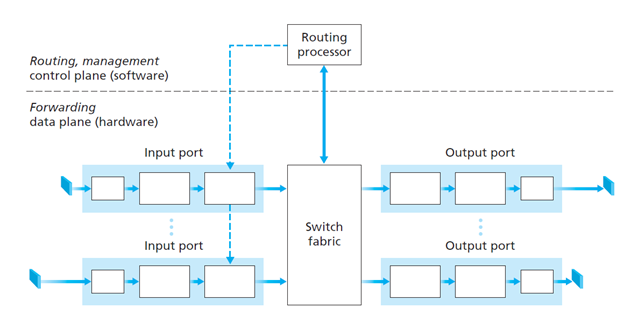
\includegraphics[scale=0.8]{cn1.png}
    \caption{Router Architecture}
    \label{fig:my_label_1}
\end{figure}

\begin{itemize}
    \item The forwarding plane is implemented entirely in hardware as software implementations will not keep up with high rates of incoming data from the input ports. (eg: with 10 Gbps link and 64 byte datagram size, each datagram has to be processed in 51.2ns. If there are $N$ ports on a single line card, then the processing time becomes $51.2/N$ ns. 
    
    \item The forwarding table lookup at the input port is sped up by more efficient searching algorithms, as well as faster memory like DRAM and SRAM (used as secondary DRAM) on the chip itself. 
    
    \item Technologies like \textbf{TCAM} (Ternary Content Access Memory) deliver $O(1)$ lookup time for a given key (in this case a 32-bit IP Address). 
    
    \item There are three main types of switching techniques:
    
    \begin{enumerate}
        \item \textit{Switching via Memory}: 
        \begin{itemize}
            \item The packets arrive at the input port, and an interrupt is sent to the routing processor.
            
            \item The packet is copied into the processor memory. Lookup is performed by extracting the header from the packet. 
            
            \item Then the packet is copied again to the buffer of the appropriate output port. 
            
            \item As only one read/write can take place at a time over the shared bus, only one packet can be switched at a time. Also if the memory bandwidth is $B$ packets per sec, then the overall switching bandwidth is less than $B/2$ packets/s. 
            
            \item In modern routers that use memory switching the forwarding computation is done in the input port itself, and the processor only handles the movement of packets to the correct output. 
        \end{itemize}
        
        \item \textit{Switching via bus}:
        \begin{itemize}
            \item The input port prepends a switch label (header) to each packet and sends it along the shared bus to all the output ports.
            
            \item The packet will be discarded by all the output ports that don't match the switch label. 
            
            \item Here too, only one packet can use the bus at a time. The switching speed is bottlenecked by the bus speed. 
            
            \item This is commonly used for small area or enterprise networks.
        \end{itemize}
        
        \item \textit{Switching via interconnection network}:
        \begin{itemize}
            \item Crossbar switches are switches that use $2N$ connections to connect $N$ output and $N$ input ports to each other. 
            
            \item \textbf{Crossbar switches} allow multiple packets to be switched in parallel, unless they are destined for the same output port, in which case they have to queue at the input. 
            
            \item \textbf{Multistage switches} are built from layers of smaller switches for further parallelism in the switching process. 
            
            \item Cisco CRS routers use \textbf{multiple switching planes} in parallel. (8 planes, each with 3 stage switching logic, totally upto 100s of Tbps switching speeds). 
        \end{itemize}
    \end{enumerate}
\end{itemize}

\begin{figure}[!h]
    \centering
    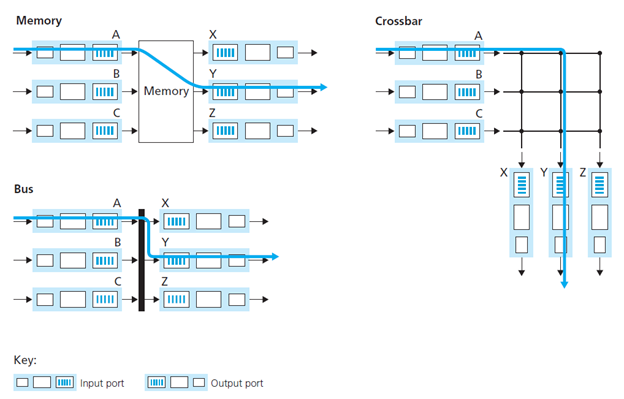
\includegraphics[scale=0.8]{cn2.png}
    \caption{Switching Technologies}
    \label{fig:my_label_2}
\end{figure}

\subsection{Queuing in Routers}
\begin{itemize}
    \item Let the input and output ports have a speed of $R_{link}$ and the switching rate be $R_{switch}$ which is $N$ times as fast as $R_{link}$. ($N$ being number of input and output ports). 
    
    \item It is assumed here that all the incoming packets are destined for one output port. 
    
    \item This setup leads to negligible queuing at the input buffer as $N$ packets can be switched through the fabric in the same time that it takes $N$ packets to arrive at all the input ports.
    
    \item At the output ports however, only one packet can be transmitted at a time. In the time that a single packet is transmitted out on the output port, there are $N$ packets arriving at that output port. 
    
    \item The packets that are not being sent out immediately must queue at the output port. 
\end{itemize}
\begin{figure}[!h]
    \centering
    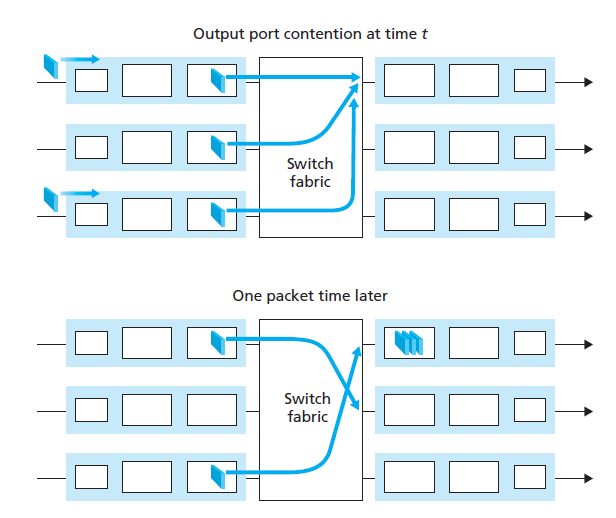
\includegraphics[scale=0.7]{cn3.png}
    \caption{Output Port Queuing}
    \label{fig:my_label_3}
\end{figure}

\begin{itemize}
    \item The ideal buffer size $B$ was for many years calculated as 
    
    \begin{equation}
        B = RTT \times C
    \end{equation}
    
    where RTT is the average round trip time for a packet and C is the link capacity. This was calculated based on analysis of a relatively smaller number of TCP flows.
    
    \item With large scale networks, this is modified to
    \begin{equation}
        B = \frac{RTT \times C}{\sqrt{N}}
    \end{equation}
    where $N$ is the number of TCP flows. 
    
    \item Too much buffer size however leads to delays, caused by longer RTTs. 
\end{itemize}

\subsubsection{Output Queue Scheduling}
\begin{itemize}
    \item The objective of this scheduling algorithm is to select one packet from the output queue for transmission. 
    
    \item Basic algorithm for this is \textbf{FCFS}, also referred to as FIFO. 
    
    \item \textbf{Priority scheduling} of packets is implemented as 2 o more queues (sorted by priority). The packets are sent out from the output queue that has buffered packets and has the highest priority. 
    
    \item In \textbf{Round Robin Scheduling}, the arriving packets are sent into queues that are based on the class of the packet. Each queue is served an equal amount of time. 
    
    \item In \textbf{Weighted Fair Queuing} (WFQ), each queue has a weight attached to it. The queue is served for a slice of time that is proportional to its weight. This policy guarantees minimum bandwidth per class of packet. 
\end{itemize}

\subsubsection{Output Queue Packet Management}
\begin{itemize}
    \item If a packet arrives at the output port and the buffer is full, then packets have to be dropped. 
    
    \item If the currently arriving packet is dropped, the policy is called \textbf{tail-drop}. 
    
    \item Packets that are currently in the queue can also be dropped on a priority basis to make room for the incoming packet. 
    
    \item Algorithms such as RED (\textit{Random Early Detection}) are used to mark packets that signify that congestion is occurring in the network.
\end{itemize}

\subsubsection{HOL Blocking}
\begin{itemize}
    \item Suppose packets at the input port are scheduled in an FCFS manner. Let there be 2 packets destined for the same output port at the head of the input queues. 
    
    \item The queued packet in an input queue must wait for transfer through the fabric (even though its output port is free) because it is blocked by another packet at the head of the line. This phenomenon is called \textbf{Head Of Line Blocking} or HOL Blocking. 
    
    \item It can be shown that HOL Blocking can cause the input queue to grow without bound, under certain assumptions, as soon as the packet arrival rate on the input links reaches only 58 percent of their capacity.
\end{itemize}

\begin{figure}[!ht]
    \centering
    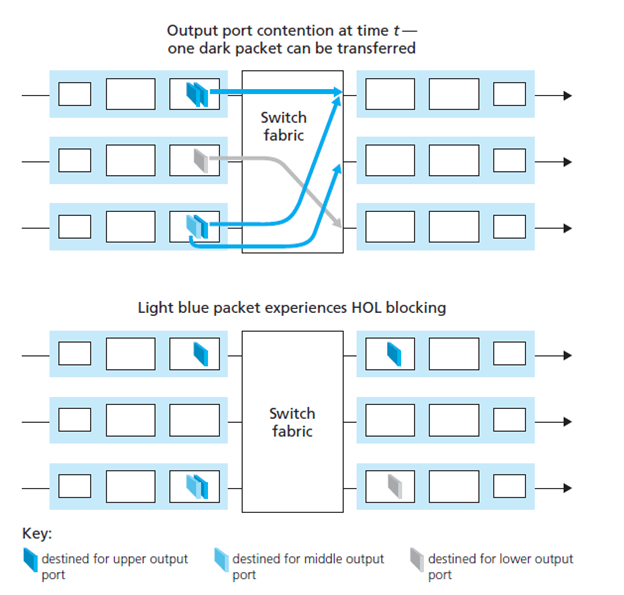
\includegraphics[scale=0.7]{cn4.png}
    \caption{Example for HOL Blocking}
    \label{fig:my_label_4}
\end{figure}

\section{Internet Protocol v4 (IPv4)}
\begin{itemize}
    \item IP is the most common network layer protocol. Its two most common functionalities are \textit{addressing} and \textit{forwarding}. 
    
    \item The network layer of TCP/IP stack has three main components: \begin{enumerate}
        \item Routing protocols to fill forwarding table entries in the routers
        
        \item IP protocol for forwarding/addressing 
        
        \item Error reporting and network layer info delivery service which is called ICMP (Internet Control Message Protocol)
    \end{enumerate}
\end{itemize}

\begin{figure}[!t]
    \centering
    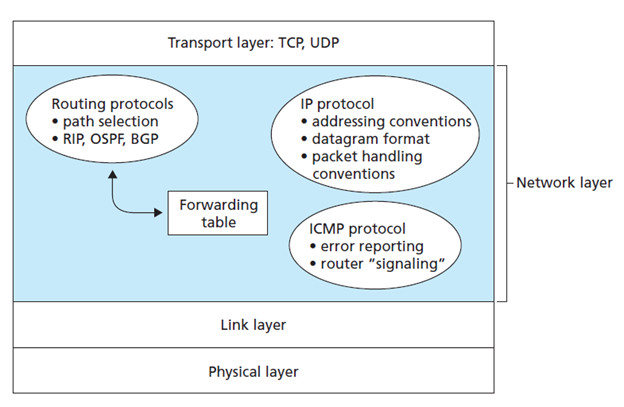
\includegraphics[scale=0.6]{cn6.png}
    \caption{Network Layer Protocols}
    \label{fig:my_label_5}
\end{figure}

\subsection{IPv4 Datagram Format}
\begin{figure}[!h]
    \centering
    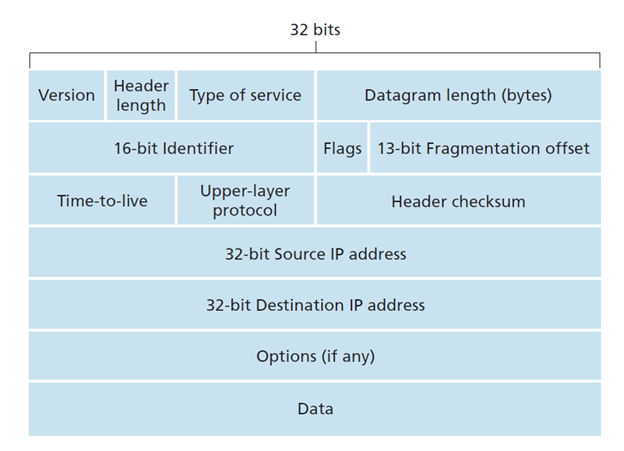
\includegraphics[scale=0.5]{cn5.png}
    \caption{IPv4 Datagram Format}
    \label{fig:my_label_6}
\end{figure}
\begin{itemize}
    \item \textit{Version Number}: 4 byte number indicating IP version (4 or 6). This indicates the rest of the datagram format.
    
    \item \textit{Header Length}: Including the options field. Without the variable-length options the IP header is 20 bytes long. 
    
    \item \textit{Type of Service} (ToS): Special requirements like low delay or high throughput for certain datagrams are indicated in this field. This distinguishes packets from services like real-time telephony from non real-time applications like FTP. The policies set by router admin indicate the implementation of these services. 
    
    \item \textit{Identifier, Flags, Frag offset}: 3 bit flags, 13 bit offset is used during IP Fragmentation used to split large IP datagrams.
    
    \item \textit{Time To Live} (TTL): To ensure that datagrams do not stay forever in the network. The TTL is decremented at each router and removed from the network with a time limit exceeded error when the TTL reaches 0.
    
    \item \textit{Upper Layer Protocol}: Value indicating transport layer protocol to which to transmit, analogous to port number in transport layer header (value 6 for TCP, 17 for UDP). 
    
    \item \textit{Header Checksum}: The header (including options) is split into words of 2 bytes (16 bits) and then the 1's complement of the sum (with carry wrapped around) is sent as the checksum. 
    
    \item \textit{Options}: Not included in version 6, the options specify information like record route taken, specify list of routers to visit, and timestamps. 
    
    \item \textit{Source and Destination IP Addresses}
\end{itemize}

\subsection{Fragmentation in IPv4}
\begin{itemize}
    \item The largest possible amount of data that a link-layer frame can carry is defined by the MTU (Maximum Transmission Unit). Each link-layer protocol has its own MTU value defined. 
    
    \item The solution to this is fragmentation, wherein the large IP Datagram is split into smaller datagrams, each of which is sent on a separate link layer frame. 
    
    \item The receiver end reassembles the fragments in order to send to the transport layer. This is done at the host system end and not in the routers. 
    
    \item The Identification, flags and offset fields help in reassembly. 
    
    \item eg: A 4000 byte datagram (20 header + 3980 content) arrives at a router. The output link has MTU of 1500 bytes (20 for IP header + 1480 data). Hence the 3980 bytes of incoming data is split into 3 chunks of 1480, 1480 and 1020 bytes.
    
    \item The offset fields are set in multiples of 8 bytes. The frag flag value is 1 for all the fragments except the last one (0 indicates the end of that IP datagram). 
    
    \item All the fragments have the same ID as the original IP datagram. 
    
    \item Fragmentation allows for the use of multiple Link layer protocols on one path. 
    
    \item Disadvantages of fragmentation:
    \begin{enumerate}
        \item Increases complexity of routers and end systems with fragmentation and reassembly hardware/software.
        
        \item Vulnerable to DDoS attacks, caused by invalid fragments inserted or invalid offset values that make fragments overlap, which make the OS crash during reassembly. 
    \end{enumerate}
\end{itemize}

\subsection{IPv4 Addressing}
\begin{itemize}
    \item IPv4 addresses are 32 bits long. They are written as 4 groups of 8 bits, each group converted to base 10 and written as a separate number separated by a dot (.)
    
    \item This notation is called the dotted decimal notation. eg: The IP Address \texttt{11000001 00100000 11011000 00001001}, it is written as \texttt{193.32.216.9} .
    
    \item Every interface on every host and router on the internet should have a globally unique IP Addresses (except for those behind NAT). 
    
    \item One portion of an IP Address is decided by the \textbf{subnet} to which that interface is connected. A subnet is a collection of computers 
    
    \item The IP Address consists of 2 parts: a subnet identifier and a host identifier. The first $n$ bits of the IP Address are subnet ID, and the last $32-n$ bits are the host ID. 
    
    \item To determine the subnets, detach each interface from its host or router, creating islands of isolated networks, with interfaces terminating the end points of the isolated networks. Each of these isolated networks is called a subnet. 
    
    \item In every subnet, the addresses \texttt{0.0.0.0} and \texttt{255.255.255.255} are reserved as broadcast addresses. 
\end{itemize}

\begin{figure}[!h]
    \centering
    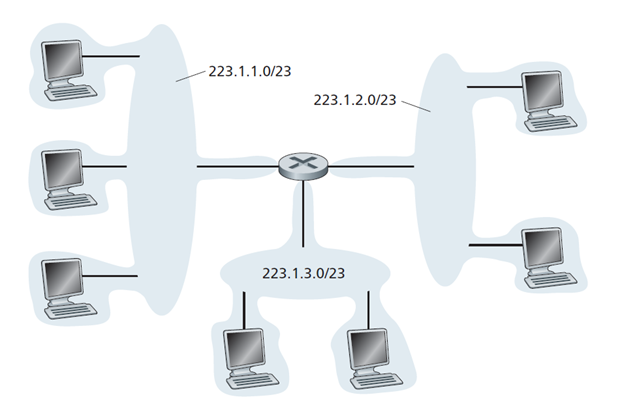
\includegraphics[scale=0.7]{cn7.png}
    \caption{Subnet Addresses}
    \label{fig:my_label_7}
\end{figure}

\begin{figure}[!h]
    \centering
    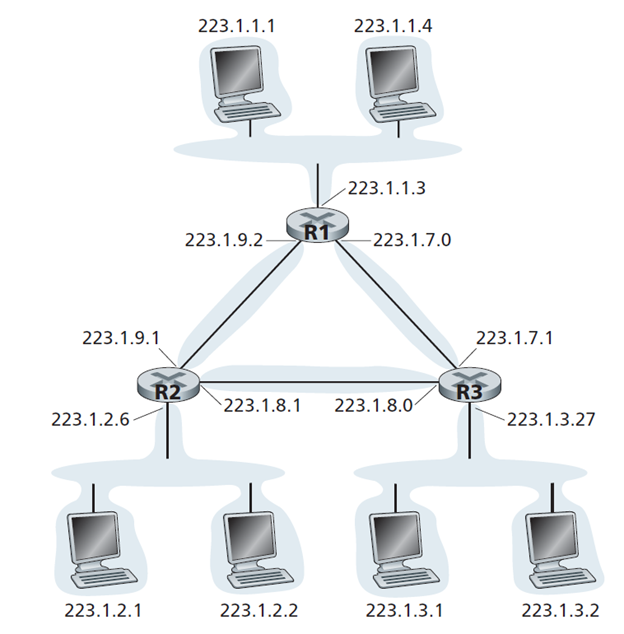
\includegraphics[scale=0.7]{cn8.png}
    \caption{Routers connecting 6 subnets}
    \label{fig:my_label_8}
\end{figure}

\begin{itemize}
    \item The notation $a.b.c.d/x$ is called \textbf{Classless Inter-Domain Routing} or CIDR. The $x$ is called the subnet mask, and indicates that the first $x$ bits of the IP Address are the subnet identifier. 
    
    \item The previous type of IPv4 addressing was called \textbf{classful addressing}. Classes A, B and C were defined as having subnet identifiers of size 8, 16 and 24 bits respectively. 
    
    \item Class A Addresses have the first octet in range 1-126, Class B addresses have range 128-191 and class C addresses have range 192-223. 
    
    \item The classful addressing scheme led to inefficient use of a limited number of IP Addresses. (eg: if a company with 2000 hosts is allocated a Class B address then there are $65536-2000 =  63534$ unused IP Addresses in that block which cannot be used by another organization). 
    
    \item Organizations obtain blocks of IP addresses from their respective ISPs. ISPs in turn obtain larger address blocks from the \textit{Internet Corporation for Assigned Names and Numbers} (ICANN). 
    
    \item ICANN handles IP address allocation as well as DNS server management and domain name allocations/disputes. ICANN allocates addresses to regional internet registries like APNIC (Asia Pacific), LACNIC (Latin America \& Caribbean), ARIN (North America), RIPE (Europe) and AFRINIC (Africa).  
    
\end{itemize}

\section{Dynamic Host Configuration Protocol (DHCP)}
\begin{itemize}
    \item This is an \textbf{application-layer} protocol that is used by host machines on a network to get IP Addresses and other details such as the DNS server's IP Address and the IP Address of the first hop router (aka the \textit{default gateway}). 
    
    \item DHCP can be configured to give the same IP address to a machine each time it connects to a network, or different \textbf{temporary} IP Addresses each time. 
    
    \item Properties of DHCP:
    \begin{enumerate}
        \item \textbf{Client-Server Protocol}: The DHCP server (often integrated into the router) maintains a list of free IP Addresses from which new ones are allocated and to which the unused ones return. 
        
        \item \textbf{Plug-and-Play Protocol}:It automates the process of IP address configuration that would otherwise have to be done manually for each system by the network admin. 
    \end{enumerate}
\end{itemize}

\subsection{4-step Process (DORA)}
\begin{itemize}
    \item \textit{Step 1}: \textbf{Discovery}
    \begin{itemize}
        \item The newly connected host searches for a DHCP server to provide it information. It does this by sending a UDP segment to \textbf{port 67 on the server}, with the IP datagram having source IP as \texttt{0.0.0.0} and destination address as \texttt{255.255.255.255}.
        
        \item The destination address \texttt{255.255.255.255} indicates that the UDP segment is to be sent to all the hosts on the network, in a process called \textit{broadcasting}. 
    \end{itemize}
    
    \item \textit{Step 2}: \textbf{Offer}
    \begin{itemize}
        \item A DHCP server receiving a broadcast discovery message replies with a message containing an IP Address, the transaction ID of the discovery message and a lease time that indicates the validity of the offered IP Address. 
        
        \item This message is also broadcast to all hosts in the network. It is sent to \textbf{UDP Port 68} on the client.  
    \end{itemize}
    
    \item \textit{Step 3}: \textbf{Request}
    \begin{itemize}
        \item The client chooses one of the offers, and sends a request message back to the server from which that offer was received. 
    \end{itemize}
    
    \item \textit{Step 4}: \textbf{Acknowledgement}
    \begin{itemize}
        \item The DHCP server replies to the request with an acknowledgement message that confirms the information sent in the offer message. 
    \end{itemize}
\end{itemize}
\begin{figure}[!h]
    \centering
    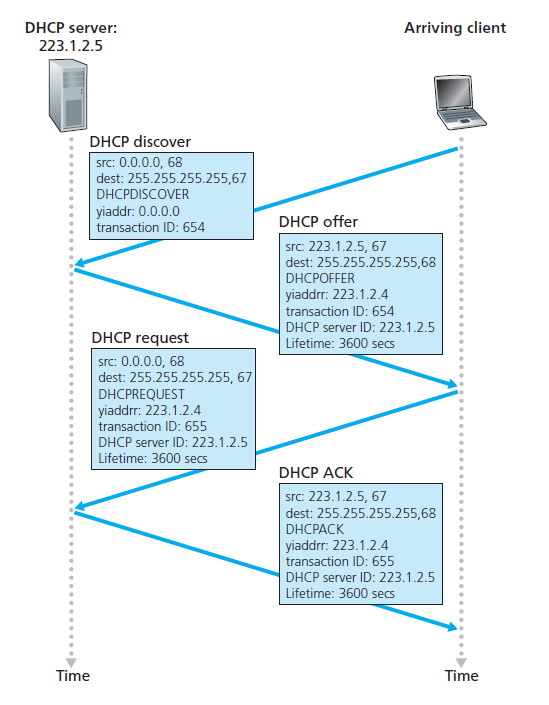
\includegraphics[scale=0.8]{cn9.png}
    \caption{DHCP Client-Server Interaction}
    \label{fig:my_label_9}
\end{figure}

\section{Network Address Translation (NAT)}
\begin{itemize}
    \item NAT is a technology that is used to map one IP Address space to another, by modifying network address information in the IP header of packets while they are in transit across a traffic routing device.
    
    \item This technique avoid the need to assign a new unique IP address to every host that joins a network, in case a network is moved or the ISP is changed. 
    
    \item In the face of IPv4 address exhaustion, NAT is now commonly used to  conserve the IP address space.
    
    \item A NAT-enabled router translates the private address of the host in the local network, to the address of the router interface that is exposed to the outside internet or WAN. 
    
    \item As all hosts in the local network appear to have the same IP Address, they are distinguished based on port numbers. 
    
    \item The following are the controversial aspects of NAT as raised by the IETF:
    \begin{itemize}
        \item The use of port numbers for addressing hosts within a private network is in opposition to the requirement that port numbers be used to address application-layer processes running on a host.
        
        \item Routers should only be restricted to managing layer 3 addresses (IP Addresses) and below. But the manipulation of IP Addresses as well as port numbers (which are layer 2 information) is in opposition to this.
        
        \item To solve the shortage of IPv4 addresses, IPv6 is meant to be used instead of NAT. 
        
        \item NAT requires network applications to be coded differently. In particular NAT affects P2P applications like file sharing and voice call applications, as these require the setup of a direct TCP connection between 2 peers.  (eg: if a peer B is behind a NAT, it cannot act as a server to accept TCP connections from A. A instead requests an intermediate C to tell B to start a TCP connection with A directly. This hack is called \textbf{connection reversal}).
    \end{itemize}
\end{itemize}

\begin{figure}[!h]
    \centering
    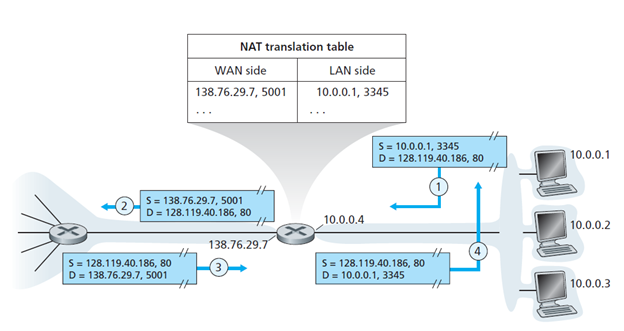
\includegraphics[scale=0.8]{cn10.png}
    \caption{Working of NAT}
    \label{fig:my_label_10}
\end{figure}

\section{Internet Control Message Protocol (ICMP)}
\begin{itemize}
    \item ICMP is the network layer's error reporting and information delivery service.
    
    \item It acts as an intermediary above the network layer, and ICMP messages are carried as IP Payloads (like TCP or UDP segments). 
    
    \item ICMP messages have a type field, a code field and contain the first 8 bytes of the IP datagram that generated that error. 
    
    \item The \texttt{ping} program sends out type 8 code 0 (echo request) messages and receives type 0 code 0 (echo response) messages in case of a successful delivery. The \texttt{ping} program is used as a network diagnostic tool.
    
    \item The source quench message (type 4 code 0) is a form of congestion control that is implemented at the network layer. It is sent out by a congested router to a host to tell that host to reduce its transmission rate. 
\end{itemize}

\subsection{Traceroute}
\begin{itemize}
    \item \texttt{traceroute} is a program that is used to determine the path taken by IP Datagrams between 2 hosts on the internet. It makes use of ICMP messages
    
    \item The sending host sends out IP datagrams that carry UDP segments having invalid port numbers, and contain TTL values of 1, 2, 3, ..., $n$.
    
    \item The $n^{th}$ router receiving the $n^{th}$ datagram sees that the TTL has just expired. It sends back an ICMP message with type 11 code 0 indicating TTL expired. 
    
    \item The TTL expired message contains the IP Address and name of the router. The source estimates the round trip time of that ICMP message from the timer, and the name/address of the router from the ICMP message. 
    \item The \texttt{traceroute} sender stops sending the IP datagrams when it receives an ICMP message of type 3 code 3 (unreachable port), as the UDP segment that was sent contains an invalid port number. 
    
    \item The client program must be able to isntruct the OS to generate IP datagrams with specific TTL values, and must be aware of the incoming ICMP messages. 
\end{itemize}

\begin{figure}
    \centering
    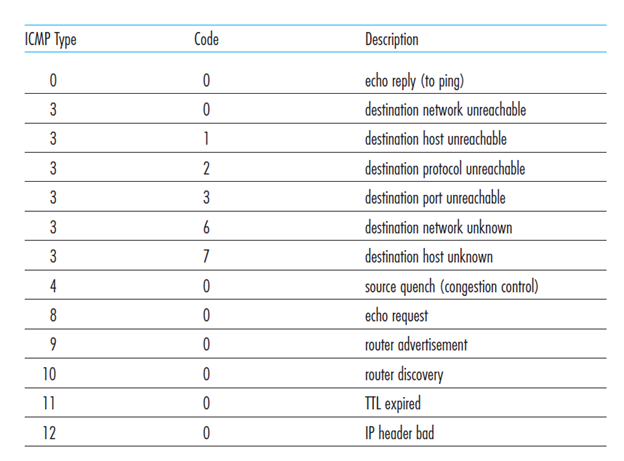
\includegraphics[scale=0.6]{cn11.png}
    \caption{ICMP type and code information}
    \label{fig:my_label_11}
\end{figure}

\section{Internet Protocol v6 (IPv6)}
\begin{itemize}
    \item IPv6 aims to solve the address space exhaustion problem that is a part of IPv4 due to its limited number of addresses ($2^{32}$) and the increasing number of hosts on the internet. 
    
    \item IPv6 also included enhanced addressing capabilities as well as other features that were learned from the experience of implementing IPv4.
\end{itemize}

\subsection{Features of IPv6}
\begin{itemize}

    \item \textit{128-bit addresses}, and a new class of addresses called \textit{anycast} addresses that allow datagrams to be transmitted to any one of a group of hosts (eg: to send an HTTP GET to the nearest of a number of mirror sites that contain a given document.)
    
    \item \textbf{Flow labelling and priority} is a new feature of IPv6 that enables labeling of packets belonging to particular flows for which the sender requests special handling, such as a non-default quality of service or real-time service. (eg: audio/video is treated as a flow, but file transfer or e-mail may not). 
    
    \item IPv6 \textbf{removes} the responsibility of \textbf{fragmentation and reassembly} from the routers and puts it only on the end systems. In case an incoming IPv6 datagram is too large to be forwarded over the next link, an "Datagram too large" ICMP message is sent back and the sender resends the datagram in smaller chunks.
    
    \item As transport layer and link layer protocols compute data checksums, the redundancy of a \textbf{header checksum was removed} from IPv4.
    
    \item The \textbf{options field} of IPv4 is \textbf{removed}, but the "next header" field in the IPv6 format points to the options that can be the next header in the IPv6 datagram just like TCP or UDP segments. 
\end{itemize}

\subsection{IPv6 Datagram Format}
\begin{itemize}
    \item \textit{Version}: 4 bit version number (1010 in this case)
    
    \item \textit{Traffic Class}: 8 bits, similar to the Type of Service field in IPv4
    
    \item \textit{Flow Label}: 20 bits to identify the flow.
    
    \item \textit{Payload Length}: 16 bits to indicate the length of the data field in the datagram (after the 40 byte header)
    
    \item \textit{Next Header}: The upper layer protocol to which the data must be delivered (value of 6 indicates TCP, 17 indicates UDP).
    
    \item \textit{Hop Limit}: Similar to a TTL field. 
    
    \item \textit{Source, Destination IP Addresses}: 128 bit IP Addresses. 
\end{itemize}

\subsection{IPv6 Addressing}
\begin{itemize}
    \item IPv6 Addresses are written as 8 groups of 4 hexadecimal digits each, separated by a colon (:). This is called the \textit{colon hexadecimal} notation.
    
    \item In each section of 4 hex digits, the leading zeros can be ignored (eg: 0A12 can be written as A12, 00FF can be written as FF and 0002 can be written as 2)
    
    \item Consecutive sections of zeros can be compressed into the double colon symbol (::). This compression can be applied only once, and can be applied anywhere on the address. 
\end{itemize}

\subsubsection{Types of IPv6 Addresses}
\begin{itemize}
    \item \textbf{Unicast Address}: Identifies a single interface on a router/host machine. 
    
    \item \textbf{Anycast Address}: It defines a group of computers that share a single address. A packet with an anycast address is delivered to the most reachable member of that group. Anycast addresses are allocated from the unicast block.
    
    \item \textbf{Multicast Address}: All members of the group of computers receive a copy of a packet that is sent to a multicast address. 
\end{itemize}

\subsection{Interface ID}
\begin{itemize}
    \item The Interface ID of a router or host interface is configured from its manufacturer-supplied MAC address (Layer 2 address). The MAC address is 48 bits in length, written as 6 groups of 2 hex digits each. 
    
    \item This is done by first inverting the 7th bit from the left of the MAC address (1 to 0 or 0 to 1). 
    
    \item Following this, the result of the above operation is split into 2 groups, the hexadecimal digits FFFE added in between to get a 64-bit Interface ID. 
    
    \item eg: For the given MAC address \texttt{F5-A9-23-14-7A-D2}, the corresponding Interface ID is written as  \texttt{F7A9:23FF:FE14:7AD2}
    
    \item If the physical address is not given as a 48-bit MAC address but instead as a 64-bit EUI address (Extended Unique Identifier), then the process is simply to invert the 7th bit from the left. 
    
    \item eg: Given the EUI \texttt{F5-A9-23-EF-07-14-7A-D2}, the interface ID is \texttt{F7A9:23EF:0714:7AD2}
\end{itemize}

\subsection{Unspecified Address}
\begin{itemize}
    \item The address \texttt{::/128} (128 0s) is called the unspecified address.
    
    \item The unspecified address is used during bootstrap when a host does not know its own address and wants to send an inquiry to find it. Since any IPv6 packet needs a source address, the host uses this address for this purpose.
    
    \item The unspecified address cannot be used as a destination address.
\end{itemize}

\subsection{Loopback Address}
\begin{itemize}
    \item The address \texttt{::1/128} is called the loopback address.
    
    \item The loopback address is used to create datagrams that do not enter the network but only go till the link layer, and then loop back till the application layer. 
    
    \item Loopback addresses are used for diagnostic purposes to test functionalities of network applications. 
\end{itemize}

\subsection{Unique Local Unicast Address}
\begin{itemize}
    \item The prefix for this block is \texttt{FC00::/7}.
    
    \item The 8th bit indicates whether the address is allocated locally or by an authority. The next 40 bits are randomly selected by the site. The random block reduces the chances of duplication of these addresses.
    
    \item The next 16 bits are the subnet ID and the next 64 bits, are the Interface ID. 
    
    \item The unique local unicast address is used for \textit{site-level} addressing. They are not routable on the global internet. 
\end{itemize}

\subsection{Link-Local Unicast Address}
\begin{itemize} 
    \item Link-local addresses have the prefix \texttt{FE80::/10}. 
    
    \item The remaining 54 bits are 0, and the next 64 bits are the Interface ID. 
    
    \item Link local addresses are used only within a single link or a network segment. They are also not routable on the global internet. 
\end{itemize}

\subsection{Global Unicast Address}
\begin{itemize}
    \item This consists of a 48-bit \textbf{global routing prefix}, a 16-bit \textbf{subnet ID} and a 64-bit \textbf{interface ID}
    
    \item The subnet ID indicates which subnet of the network the host belongs to. The first subnet has an ID of 0000, the second has ID 0001 and so on. 
\end{itemize}


\subsection{Autoconfiguration}
\begin{itemize}
    \item The host first creates a link local address for itself as described above (\texttt{FE80::} followed by 54 zeros and the 64 bit interface id).
    
    \item The host verifies the uniqueness of the link-local address by sending out a \textit{neighbour solicitation} message, waiting for the reply in the form of a\textit{ neighbour advertisement} message. If the link-local address is not unique, the procedure fails and the host must use DHCP to get an IPv6 address. 
    
    \item The host sends a \textit{router solicitation} message, and waits for a \textit{router advertisement} message. The router advertisement message contains the 48-bit global routing prefix and the 16-bit subnet ID. From these 2 and the 64-bit interface ID, the global unicast address of the host is generated. 
    
    \item If the router cannot help with the process of autoconfiguration, then this is informed by setting a flag bit in the router advertisement message. 
\end{itemize}

\subsection{Renumbering}
\begin{itemize}
    \item Renumbering is a scheme that allows the global routing prefix (first 48 bits of the IPv6 address) to change. 
    
    \item This is useful when a network's service provider changes. The router now advertises this new routing prefix, but allows the use of the old prefix for a short while before disabling it. 
    
    \item Therefore for a short period during transition, the network has two valid global routing prefixes. 
    
    \item One issue with renumbering is the working of DNS which must also be made aware of the new routing prefixes and associate those with the domain names. A next generation DNS protocol is being created to provide support for this. 
\end{itemize}

\subsection{Transition between IPv4 and IPv6}
\subsubsection{Dual Stack Approach}
\begin{itemize}
    \item In this approach, all IPv6 nodes also have a complete IPv4 implementation inside. These nodes have both IPv4 and IPv6 addresses, and they can create both types of datagrams. 
    
    \item In order to know whether a neighbouring system is IPv4 or IPv6 capable, DNS is used. DNS returns an IPv4 address for an IPv4 compatible machine and likewise for IPv6. This means that the node issuing the request itself must be IPv6 compatible, or else DNS will only return IPv4 addresses. 
    
    \item In the below figure, since the nodes C and D are IPv4 compatible only, the extra information carried in IPv6 headers coming from B (eg: flow labels) is removed and not sent to the other IPv6 compatible nodes E and F. 
\end{itemize}

\begin{figure}[!h]
    \centering
    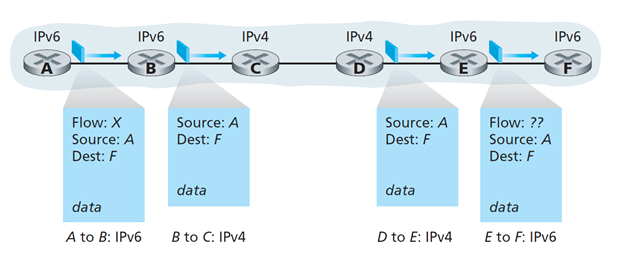
\includegraphics[scale=0.7]{cn13.png}
    \caption{Dual Stack Approach}
    \label{fig:my_label_13}
\end{figure}

\subsubsection{Tunnelling}
\begin{itemize}
    \item If an IPv6 node is connected to another IPv6 node via only an IPv4 node, the intervening IPv4 node is viewed as a tunnel.
    
    \item Through this tunnel, the entire IPv6 datagram is attached as data of an IPv4 datagram and sent across the IPv4 node, to the IPv6 node where it is decapsulated to get the actual IPv6 datagram. 
    
    \item The IPv4 datagram is addressed to the IPv6 node at the other end of the tunnel. It is routed among the IPv4 nodes till it reaches there. 
    
    \item The IPv6 node at the end of the tunnel must check the incoming IPv4 datagram to see if ti contains a valid IPv6 datagram addressed to it. 
    
    \item Upon receipt of such an IPv6 datagram it can route it through the IPv6 network like any other datagram.  
\end{itemize}

\begin{figure}[!ht]
    \centering
    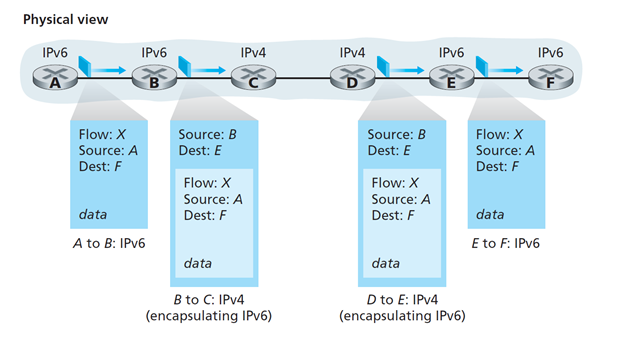
\includegraphics[scale=0.7]{cn14.png}
    \caption{Tunnelling}
    \label{fig:my_label_14}
\end{figure}

\section{Introduction to Routing Algorithms}
\begin{itemize}
    \item The primary types of routing protocols are Interior Gateway Protocols and Exterior Gateway Protocols. 
    
    \item Interior Gateway Protocols are used for exchanging routing information between gateways (commonly routers) \textit{within} an autonomous system (for example, a system of corporate local area networks). 
    
    \item The types of IGPs are \textbf{Distance-Vector} and \textbf{Link-State} routing protocols. 
    
    \item Exterior Gateway Protocols are used for exchanging routing information \textit{between} autonomous systems of routers. 
    
\end{itemize}

\begin{figure}[!h]
    \centering
    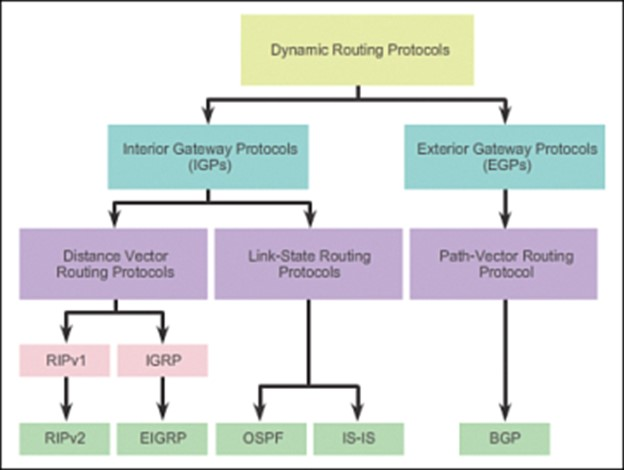
\includegraphics[scale=0.6]{cn15.jpg}
    \caption{Classification of Routing Algorithms}
    \label{fig:my_label_15}
\end{figure}

\break 

\subsection{Comparison between Distance-Vector and Link-State}
\begin{figure}[!h]
    \centering
    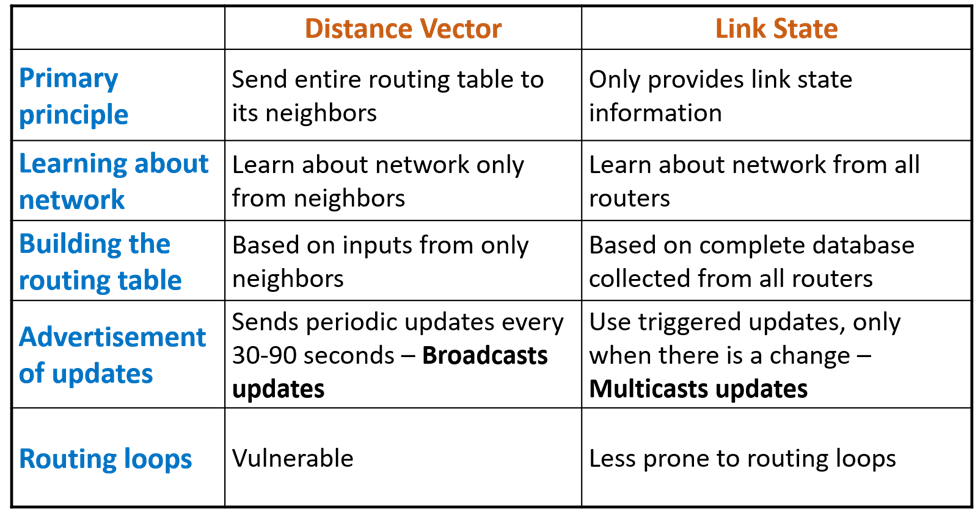
\includegraphics[scale=0.7]{cn16.png}
    \label{fig:my_label_16}
\end{figure}

\begin{figure}[!h]
    \centering
    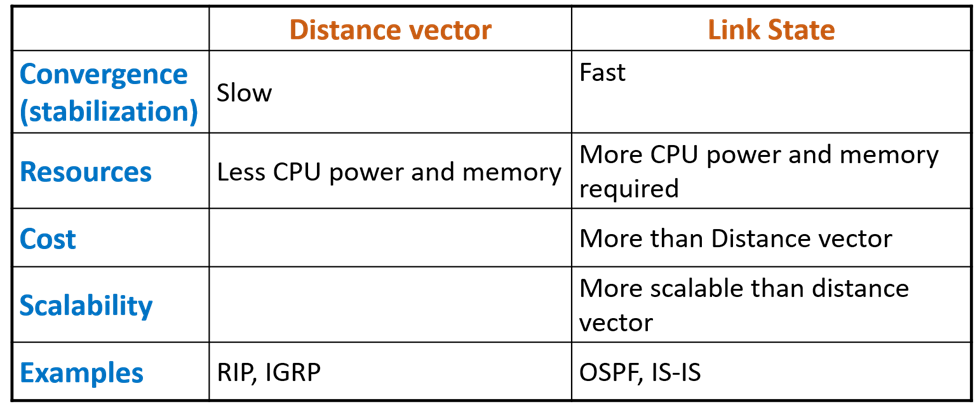
\includegraphics[scale=0.7]{cn17.png}
    \label{fig:my_label_17}
\end{figure}

\end{document}